% !TEX root = thesis-ex.tex


Hard scatterings in the colliding nuclei result in the production of highly energetic partons that evolve, decay, and eventually form conical sprays of particles called jets. Jet production is well understood in a \pp\ collision environment (where there are no QGP effects) in the context of perturbative QCD \cite{161}. In heavy ion collisions, jets must traverse the quark gluon plasma. This can result in the jet losing energy and forward momentum \cite{162, 163}, while also picking up momentum transverse to the parton direction. Jets can also deposit energy in the medium, creating a wake \cite{71, 70}. 

Jet production shown in Figure~\ref{fig:feynman_jet} can be written in terms of the parton distribution functions, scattering cross sections, and the fragmentation functions as

\begin{align}
d \sigma_{pp \rightarrow hX} \approx & \sum_{abjd} \int dx_a \int dx_b \int dz_j f_{a/p} (x_a, \mu_f) \times f_{b/p} (x_b, \mu_f) \\
& \times d\sigma_{ab\rightarrow jd} (\mu_f, \mu_F, \mu_R) \\
& \times D_{j \rightarrow h} (Z_j, \mu_f)
\end{align}

\begin{figure}[htbp]
\begin{center}
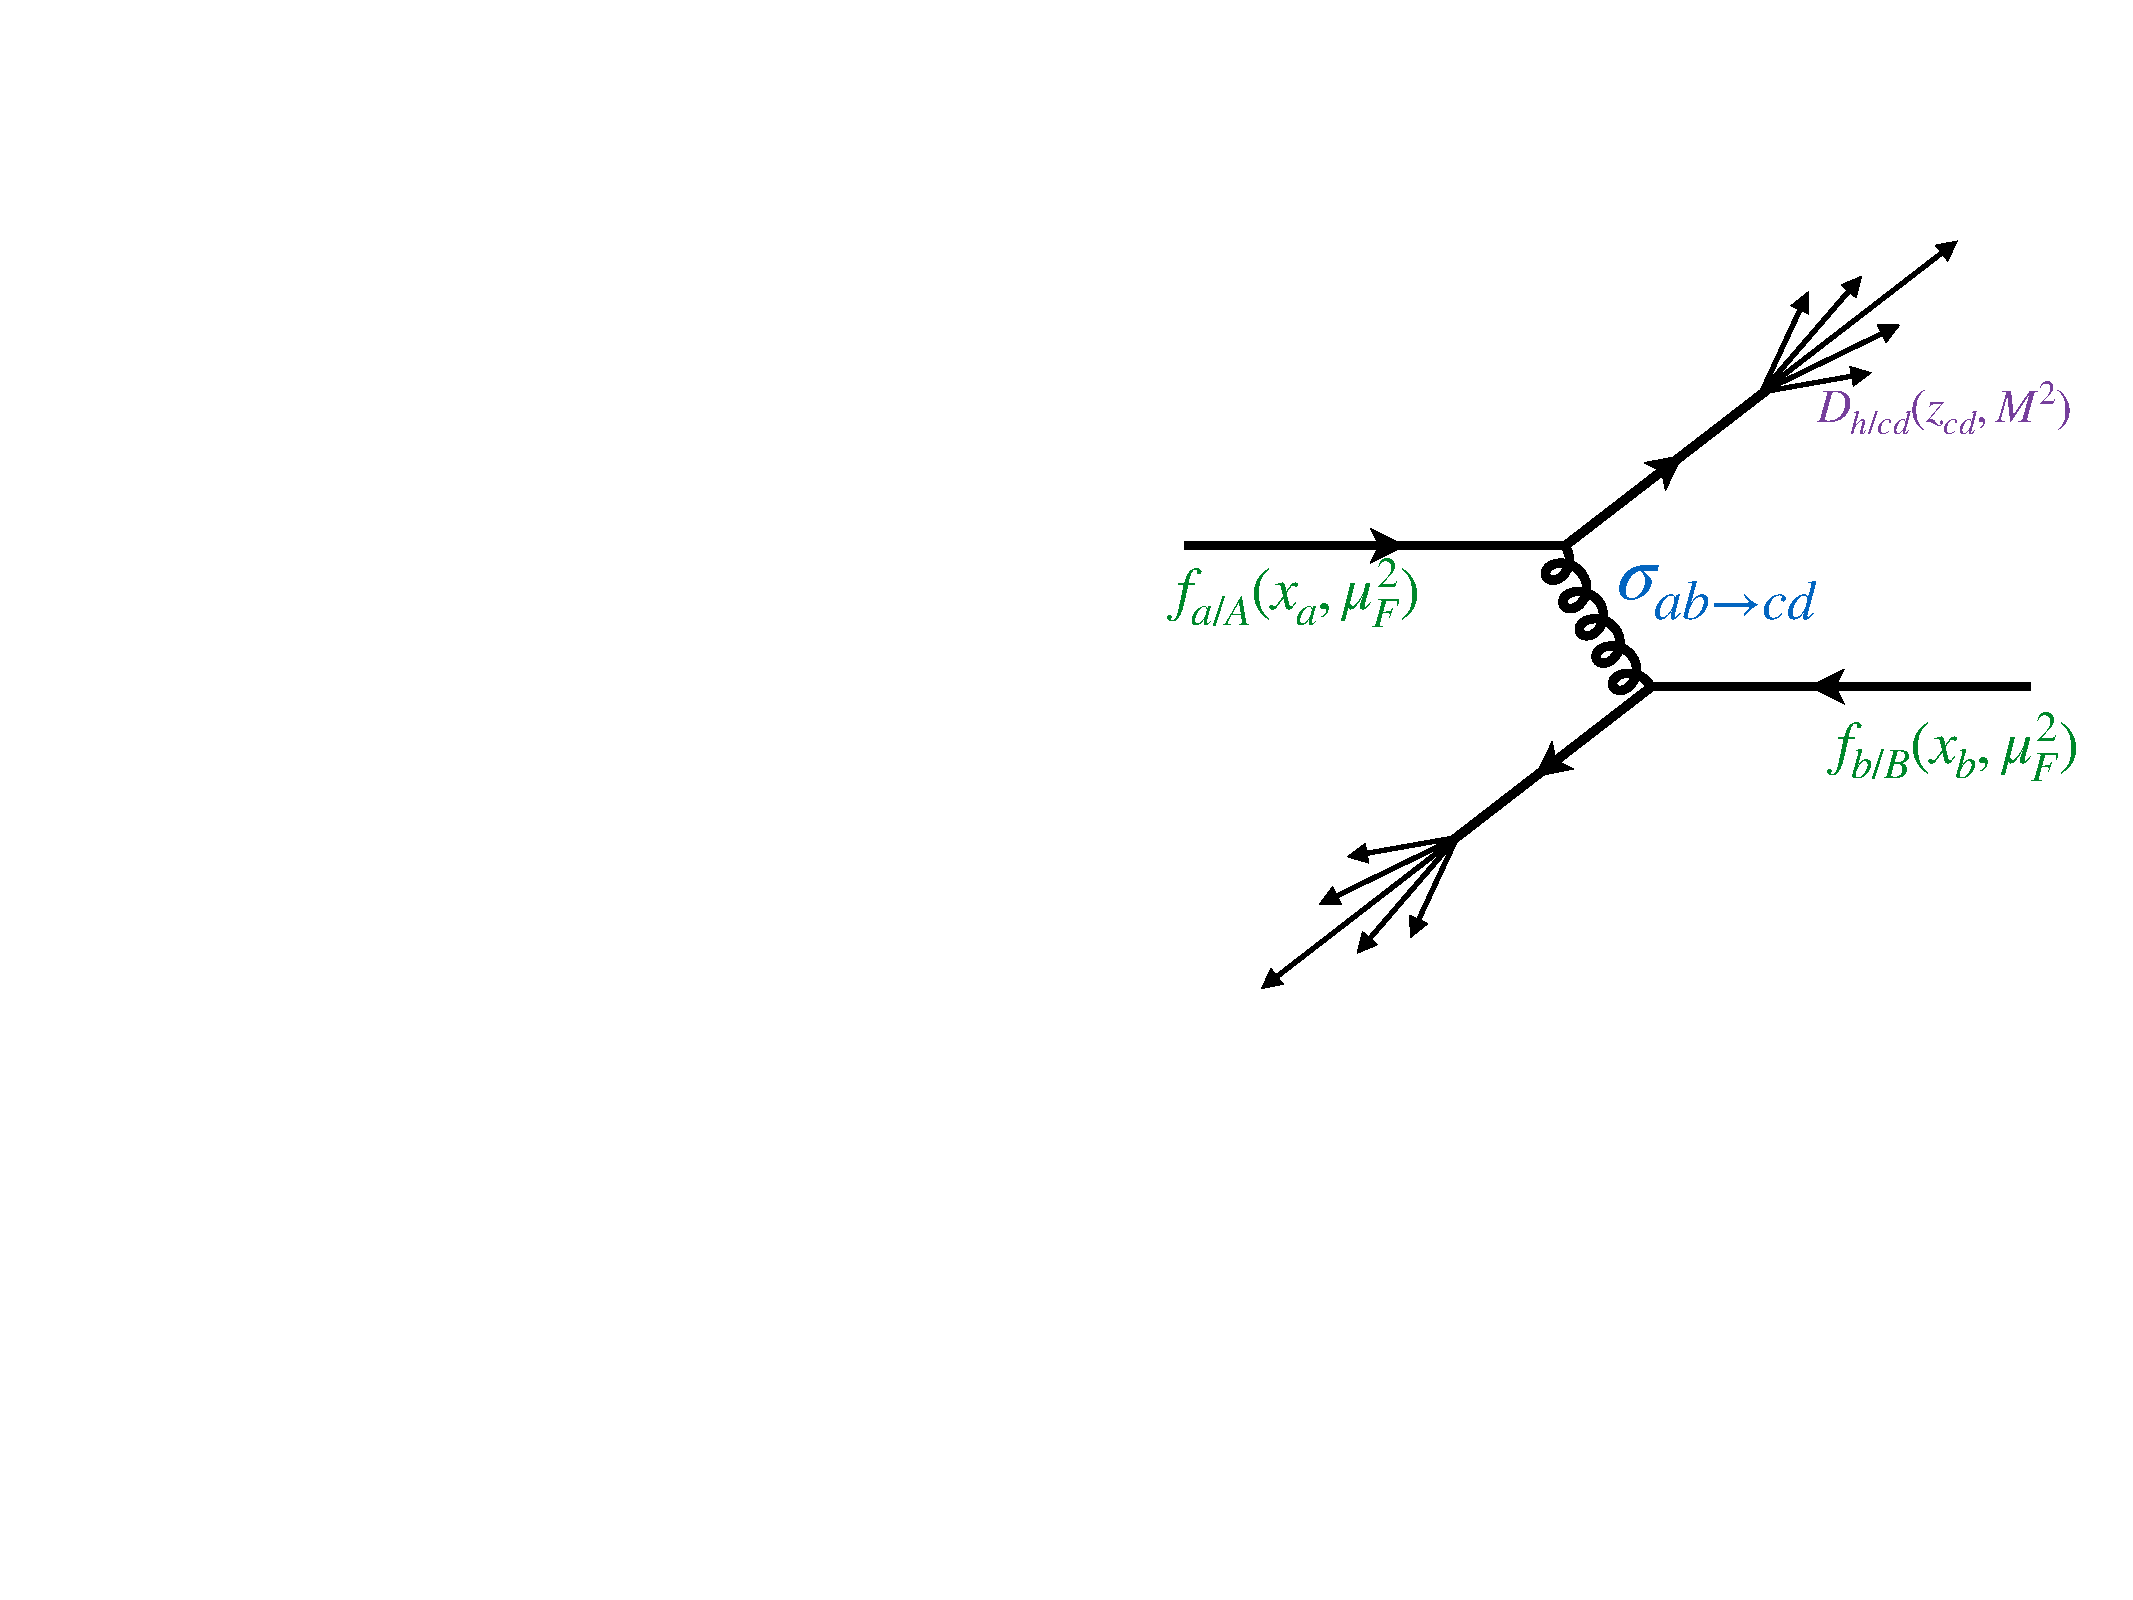
\includegraphics[width=0.55\textwidth]{figures/theory/feynman_jet}
\caption{Jet production from the process $pp \rightarrow hX$, factorizing in terms of the parton distribution functions, scattering cross sections, and jet fragmentation functions. \cite{arXiv:1511.00790}}
\label{fig:feynman_jet}
\end{center}
\end{figure}


 These are discussed in Section~\ref{sec:jets}. 


